\documentclass[a4paper,14pt]{extarticle} %the default article class is limited to 12pt, but you can go up to 14, 17 or 20 points if you use the extarticle class:
\usepackage{cmap} %make LaTeX PDF output copy-and-pasteable
\usepackage[T2A]{fontenc}
\usepackage[utf8]{inputenc}
\usepackage[english,ukrainian]{babel}

\usepackage{amssymb,amsfonts,amsmath,cite,enumerate,float}
\usepackage{indentfirst} %set an additional space before a paragraph at the begining of new section
\usepackage{setspace}
\usepackage{textcomp}

\usepackage{geometry} 
\geometry{left=1.25cm}
\geometry{right=1.25cm}
\geometry{top=1cm}
\geometry{bottom=2cm}

\usepackage{graphicx}
\usepackage{wrapfig}
\graphicspath{{images/}} %path to images

\parskip=1mm %space between paragraphs

\usepackage[dvipsnames]{xcolor}
\usepackage{color}
% 1) tutorial about xcolor:  https://www.overleaf.com/learn/latex/Using_colours_in_LaTeX
% 2) huge tutorial about xcolor: https://latex-tutorial.com/color-latex/ 
% 3) RGB calculator: https://www.w3schools.com/colors/colors_rgb.asp

\usepackage{listings} %for code

\lstset{
    frame=single, %lines
    language=Python,
    aboveskip=3mm,
    belowskip=3mm,
    columns=flexible,
    basicstyle={\small\ttfamily},
    numbers=left,
    numberstyle=\tiny\color{gray},
    commentstyle=\color{OliveGreen},
    stringstyle=\color{Mahogany},
    morestring=[b]''',
    showstringspaces=false,
    keywordstyle=\bfseries\color{Blue},
    emph={[1]import, as, for, return}, emphstyle={[1]\color{DarkOrchid}},
    emph={[2]range, abs, plot_scatter_7points, Cubic_Bezier_curve_7points, Catmull_Rom_spline_interpolation,
    Cubic_Beta_Spline_curve, Elementary_Beta_spline_curve, plot_scatter_4points, 
    Cubic_Bezier_curve_4points}, emphstyle={[2]\color{Sepia}},
    breaklines=true,
    breakatwhitespace=true,
    tabsize=4
}

\begin{document}

\begin{titlepage}
    \newpage

    \begin{minipage}[c]{\linewidth}

        \newlength{\maxpreambula}
        \settowidth{\maxpreambula}{\small{<<Київський політехнічний інститут імені Ігоря Сікорського>>}}    

        \hspace{5cm}\parbox{\maxpreambula}{
            \begin{spacing}{1.1}\small{
                Міністерство освіти і науки України \\
                Національний технічний університет України \\
                <<Київський політехнічний інститут імені Ігоря Сікорського>> \\
                Навчально-науковий фізико-технічний інститут }
            \end{spacing}
        }
            
        \vspace*{-2.35cm}
        \hspace*{1.5cm}
        
\includegraphics[width=0.13\paperwidth]{kpi_emblem.png}

    \end{minipage}
    
    \vspace{\fill}
    
    \begin{center}
        \begin{spacing}{1.5}
            \textbf{\Large{Реалізація EM-алгоритму}} \\ 
            \vspace{1cm}\textbf{\normalsize{предмет <<Марковські моделі та їхнє застосування>>}}
        \end{spacing}
    \end{center}
    
    \vspace{\fill}
    
    \newlength{\maxname}
    \settowidth{\maxname}{\small{Цибульник Антон Владиславович}}

    \hfill\parbox{\maxname}{
        \begin{spacing}{1.1}
            \small{\textbf{Роботу виконав:}} \\ 
            \small{Студент групи ФІ-91,} \\
            \small{Цибульник Антон Владиславович} \\
        \end{spacing}
    }

    \hfill\parbox{\maxname}{
        \begin{spacing}{1.1}
            \small{\textbf{Роботу перевірила:}} \\ 
            \small{Ніщенко Ірина Іванівна} \\
        \end{spacing}
    }

    \vspace{0.5cm}

    \begin{center}
        \small{2022}
    \end{center}
    
\end{titlepage}

\newpage

\subsection*{Мета}
Навчитись будувати різні види сплайнових кривих для заданого масиву опорних точок.
Виконати дослідження залежності виду кривої Безьє від порядку слідування опорних точок.

\subsection*{Теоретичні відомості} 
Сплайн -- крива, яка використовується для апроксимації заданих базових (опорних) точок. Існує велика кількість 
сплайнових кривих, які відрізняються своїми властивостями. Нехай на площині заданий упорядкований набір точок 
$P_0, \dots, P_m$. Тоді ламана $P_0, \dots, P_m$ називається контрольною ламаною, що породжена заданим масивом 
$P = \{P_0, P_1,\dots,P_m\}$. Для побудови сплайнової кривої для набору точок $P_0, \dots, P_m$ виконують 
такий алгоритм:
\begin{enumerate}
    \item[1)] Для побудови кривої на проміжку між точками $P_i, P_{i+1}$ беруть четвірку точок $P_{i-1},P_i,P_{i+1},P_{i+2}$;
    \item[2)] Задають діапазон зміни параметра $0 \leqslant t \leqslant 1$. Значення параметра $t=0$ відповідає 
    початковій точці, а $t=1$ -- кінцевій точці на ділянці кривої між точками $P_i, P_{i+1}$. Значення $0<t<1$
    відповідають внутрішнім точкам даної ділянки;
    \item[3)] Розбивають діапазон зміни параметра $t$ на $n$ частин (наприклад, $n=10$);
    \item[4)] На основі значень відповідних координат четвірки базових точок й значень $t_k, k = \overline{0,n}$,
    розраховуються $n$ проміжних точок сплайнової кривої між базовими точками $P_i, P_{i+1}$;
    \item[5)] Розраховані на попередньому кроці точки з'єднуються прямими лініями. Таким чином, чим вище значення $n$, 
    тим більш точно буде апроксимована сплайнова крива;
\end{enumerate}

Для побудови складної сплайнової кривої, що починається в першій базовій точці та закінчується в останній 
базовій точці, достатньо доповнити набір копіями першої та останньої точок. Копія першої точки при цьому 
додається в початок набору, а копія останньої точки -- в кінець набору.

\subsection*{Види сплайнових кривих}

\begin{enumerate}
    \item Інтерполяційна крива Catmull-Rom: 
    \[ r(t)=\frac{1}{2}\left( -t(1-t)^2P_0 + (2-5t^2+3t^3)P_1 + t(1+4t-3t^2)P_2 - t^2(1-t)P_3 \right) \]
    \item Кубічна крива Безьє (для чотирьох контрольних точок):
    \[ r(t)=(1-t)^3 P_0 + 3t(1-t)^2 P_1 + 3t^2(1-t) P_2 + t^3 P_3 \]
    \item Кубічна B-сплайнова крива:
    \[ r(t)=\frac{1}{6}\left( (1-t)^3 P_0 + (3t^3-6t^2+4)P_1 + (-3t^3+3t^2+3t+1)P_2 + t^3 P_3 \right) \]
    \item Елементарна B-сплайнова крива:
    \begin{align*}
        &r(t)=b_0(t)P_0 + b_1(t)P_1 + b_2(t)P_2 + b_3(t)P_3,\ \text{де} \\
        &b_0(t)=\frac{1}{\delta}\left( 2\beta_1^3(1-t)^3 \right), \\
        %&b_1(t)=\frac{1}{\delta}\left( 2\beta_1^3t(t^2-3t+3) + 2\beta_1^2(t^3-3t+2) + 2\beta_1(t^3-3t+2) + \beta_2(2t^3-3t^2+1) \right) \\
        &b_1(t)=\frac{2\beta_1^3t(t^2-3t+3) + 2\beta_1^2(t^3-3t+2) + 2\beta_1(t^3-3t+2) + \beta_2(2t^3-3t^2+1)}{\delta}, \\
        &b_2(t)=\frac{1}{\delta}\left( 2\beta_1^2t^2(3-t) + 2\beta_1t(3-t^2) + 2\beta_2t^2(3-3t) + 2(1-t^3)  \right), \\
        &b_3(t)=\frac{2t^3}{\delta}, \\ \\
        &\beta_1\geqslant 0,\ \beta_2\geqslant 0,\ \delta=2\beta_1^3 + 4\beta_1^2 + 4\beta_1 + \beta_2 + 2. 
    \end{align*}
\end{enumerate}

\subsection*{Завдання}

\begin{enumerate}
    \item На координатній площині задано масив опорних точок $P_0, P_1, P_2, P_3, P_4, P_5, P_6$. 
    Скласти програму побудови таких сплайнових кривих:
    \begin{itemize}
        \item інтерполяційна крива Catmull-Rom;
        \item кубічна крива Безьє;
        \item кубічна B-сплайнова крива;
        \item елементарна B-сплайнова крива (поексперементувати з $\beta_1,\ \beta_2$).
    \end{itemize}

    Зауваження: координати опорних точок задані в пікселах відносно початку координат, що знаходиться у лівому 
    нижньому куту поверхні екрана, на яку повинна проектуватися площина розміром $200\times 100$ умовних математичних одиниць.
    
    \subsubsection*{Вимоги до програми}

    Кожна програма повинна будувати:
    \begin{itemize}
        \item[--] контрольну ламану лінію (штрихову), що з’єднує точки в порядку їх проходження;
        \item[--] сплайнові криві для відповідної комбінації точок. 
    \end{itemize}

    Програма повинна виконувати розмітку та оцифровку області побудови сплайнових кривих з кроком 10 умовних математичних одиниць.

    \item Скласти програму побудови кубічних кривих Безьє для кожної з 6-ти комбінацій (порядку слідування) 
    опорних точок: $P_1P_2P_3P_4$, $P_1P_2P_4P_3$, $P_1P_3P_2P_4$, $P_1P_3P_4P_2$, $P_1P_4P_2P_3$, $P_1P_4P_3P_2$.
    
    Зауваження: координати опорних точок задані в пікселах відносно початку координат, що розміщений у лівому 
    нижньому куті області побудови зображення, на яку повинна проецируватися площина розміром $200\times 100$ 
    умовних математичних одиниць.

    \subsubsection*{Вимоги до програми}
    
    Кожна програма повинна будувати:

    \begin{itemize}
        \item[--] кожну криву Безьє в окремому вікні виводу, для чого весь екран слід розбити штриховими 
        лініями на 6 областей (по 3 області в 2-х рядках);  
        \item[--] в кожному випадку програма повинна будувати контрольні відрізки (штриховою лінією), що 
        з’єднують опорні точки в порядку їх проходження в кожній комбінації та відповідні підписи 
        $P_1$, $P_2$, $P_3$, $P_4$ біля точок.
    \end{itemize}

    Програма повинна виконувати розмітку та оцифровку області побудови сплайнових кривих з кроком 10 умовних математичних одиниць.

\end{enumerate}

\subsection*{Код програми й скріншоти результатів}

\subsubsection*{Чотири різних види сплайнових кривих}
\lstinputlisting{splines.py}

\newpage
\subsubsection*{Скріншоти сплайнових кривих}

\begin{figure}[h]
    \center{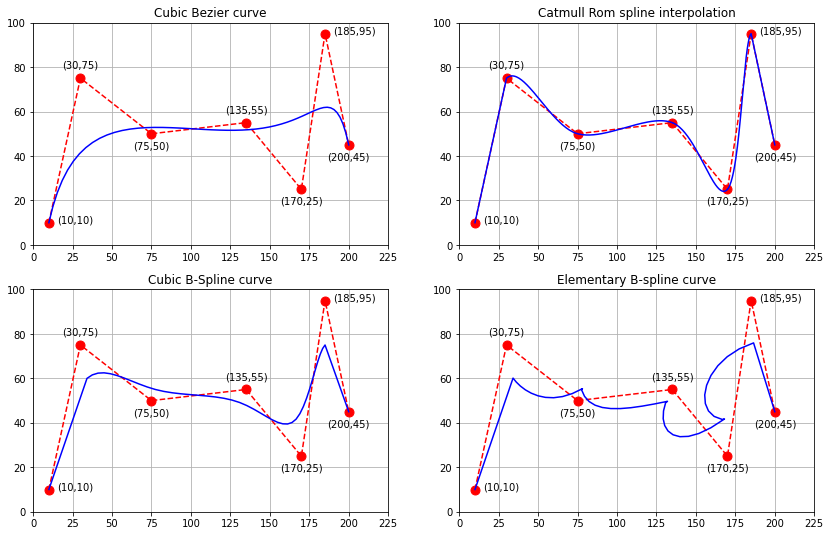
\includegraphics[width=1\linewidth]{splines.png}}
\end{figure}

\subsubsection*{Дослідження залежності виду кривої Безьє}
\lstinputlisting{Bezier curves.py}

\subsubsection*{Скріншоти кривих Безьє}

\begin{figure}[h]
    \center{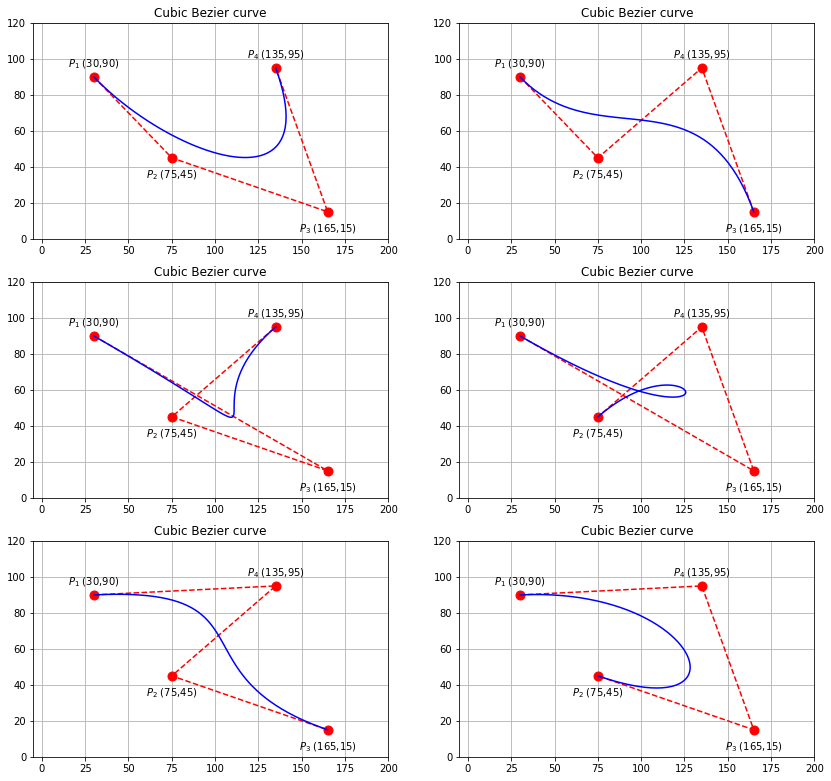
\includegraphics[width=1\linewidth]{Bezier.png}}
\end{figure}

\subsection*{Висновки}

У лабораторному практикумі я навчився будувати такі чотири різних типи сплайнових кривих: інтерполяційна крива 
Catmull-Rom, кубічна крива Безьє, кубічна B-сплайнова крива та елементарна B-сплайнова крива. Здобув практичні 
навички кодування побудови кривих на мові python. Крім того, засвоїв чимало нових елементів графічної бібліотеки 
побудови графіків \texttt{matplotlib}. Намалював графіки сплайнових кривих й зобразив усі проміжні результати на скріншотах.

\subsection*{Контрольні питання}

\begin{enumerate}

    \item \textit{Що таке сплайни? Де застосовуються сплайни?}

    Як і алгоритм цифрового диференціального аналізатора, алгоритм Брезенхейма теж використовують для пошуку 
    оптимальних растрових координат для представлення відрізку між двома точками.

    \item \textit{Які сплайнові криві ви знаєте? Яким умовам повинні задовольняти сплайни?}

    Як і алгоритм цифрового диференціального аналізатора, алгоритм Брезенхейма теж використовують для пошуку 
    оптимальних растрових координат для представлення відрізку між двома точками.

    \item \textit{Як побудувати складену сплайнову криву?}

    Як і алгоритм цифрового диференціального аналізатора, алгоритм Брезенхейма теж використовують для пошуку 
    оптимальних растрових координат для представлення відрізку між двома точками.

    \item \textit{Назвіть властивості складеної сплайнової кривої Catmull-Rom.}

    Як і алгоритм цифрового диференціального аналізатора, алгоритм Брезенхейма теж використовують для пошуку 
    оптимальних растрових координат для представлення відрізку між двома точками.

    \item \textit{Назвіть властивості кривих Безьє. Які переваги і недоліки кривих Безьє?}
    
    Як і алгоритм цифрового диференціального аналізатора, алгоритм Брезенхейма теж використовують для пошуку 
    оптимальних растрових координат для представлення відрізку між двома точками.
    
    \item \textit{Назвіть властивості кубічних B-сплайнів.}
    
    Як і алгоритм цифрового диференціального аналізатора, алгоритм Брезенхейма теж використовують для пошуку 
    оптимальних растрових координат для представлення відрізку між двома точками.

    \item \textit{Назвіть властивості складених елементарних B-сплайнових кривих.}
    
    Як і алгоритм цифрового диференціального аналізатора, алгоритм Брезенхейма теж використовують для пошуку 
    оптимальних растрових координат для представлення відрізку між двома точками.

\end{enumerate}

\end{document}